\section{Modeling}
\label{sec:modeling}


% %
% SYSTEM DESCRIPTION
% %
We consider the environment depicted in Figure \ref{fig:modeling-system-sketch}, consisting of:

\begin{itemize}
	\item  \textbf{workload:} mobile devices send to the system tasks that can be partitioned in two classes, according to their arrival rate and service demand.
	\item \textbf{system:} a two-tiers system, made of:	
	\begin{itemize}
		\item a Cloudlet with $N$ servants.
		\item a remote Cloud server with virtually unlimited servants.
		\item a front-dispatcher, responsible to route requests to Cloudlet or Cloud, according to the policy defined in Algorithm \ref{alg:modeling-dispatching-policy}, that takes into account the number $n_{clt}$ of tasks in Cloudlet, the number $n_{cld}$ of tasks in Cloud and a threshold $S$.
	\end{itemize}
\end{itemize}

\begin{figure}
	\label{fig:modeling-system-sketch}
	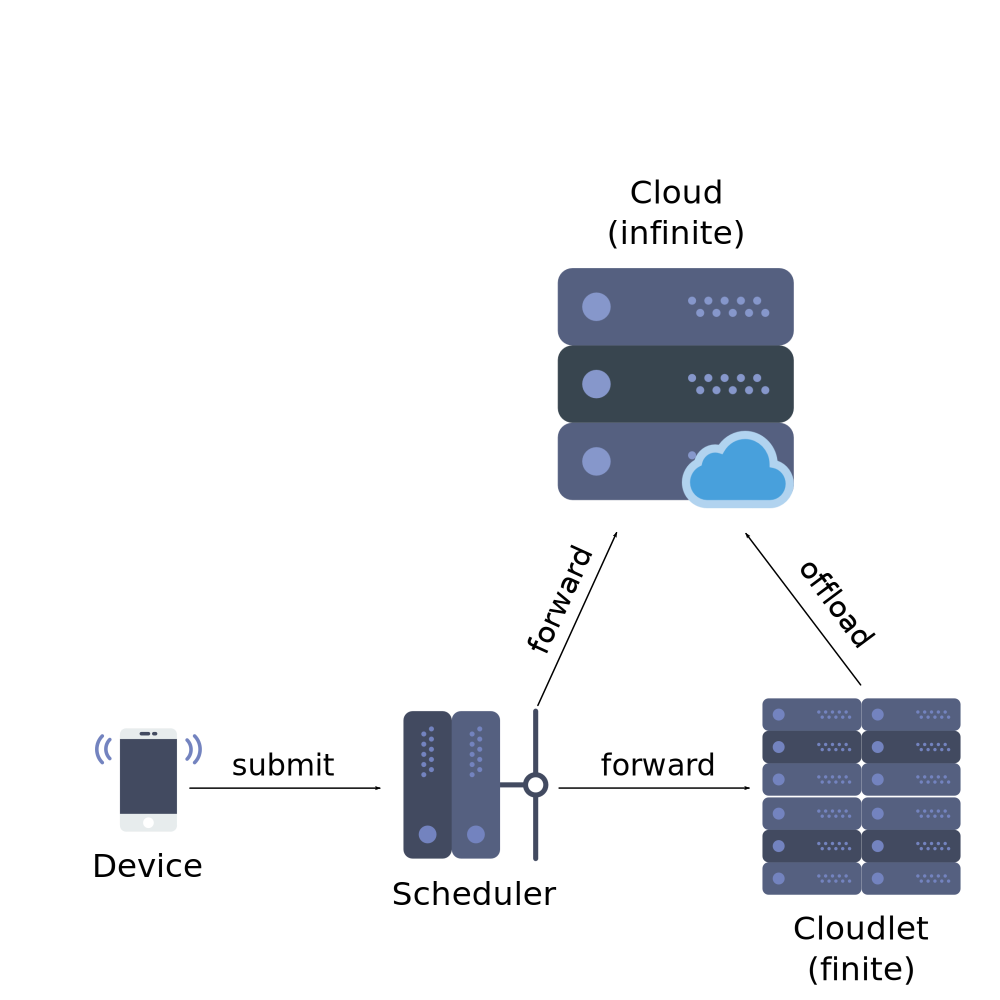
\includegraphics[width=\columnwidth]{fig/modeling-system-sketch}
	\caption{The system sketch.}
\end{figure}

We assume that 
(i) the service time includes the transmission overhead,
(ii) the Cloud provides tasks with higher service rate than the Cloudlet, 
(iii) when a task is interrupted in the Cloudlet and it is sent to the Cloud, the restart process comes with a setup time overhead.

\begin{algorithm}
	\label{alg:modeling-dispatching-policy}
	\SetAlgoLined
	\If{task of class 1}{
		\If{$n_{clt}=N$}{
			send on the Cloud
		} 
		\If{$n_{clt}+n_{cld}<S$}{
			accept
		} 
		\eIf{$n_{cld} > 0$}{
			accept the task on the Cloudlet and send a class 2 task on the Cloud
		}{
			accept the task on the Cloudlet
		}
	}
	\If{arrival of class 2}{
		\eIf{$n_{clt}+n_{cld}>=S$}{
			send on the Cloud
		}{
			accept the task on the Cloudlet
		}
	}
	\caption{The dispatching policy.}
\end{algorithm}


% %
% GOALS AND OBJECTIVES
% %
\paragraph{Goals and Objectives}
The main goals of the simulation are about system tuning.
In particular, we propose to determine with a $95\%$ level of confidence
(i) the response time as a function of the threshold $S$,
(ii) the throughput as a function of the threshold $S$,
(iii) the distribution of the response time when $S=N$ and
(iv) the threshold $S^{*}$ that minimizes the response time.

% %
% CONCEPTUAL MODEL
% %
\paragraph{Conceptual Model}
The conceptual model is depicted in Figure\ref{fig:modeling-conceptual-model}.
\begin{figure}
	\label{fig:modeling-conceptual-model}
	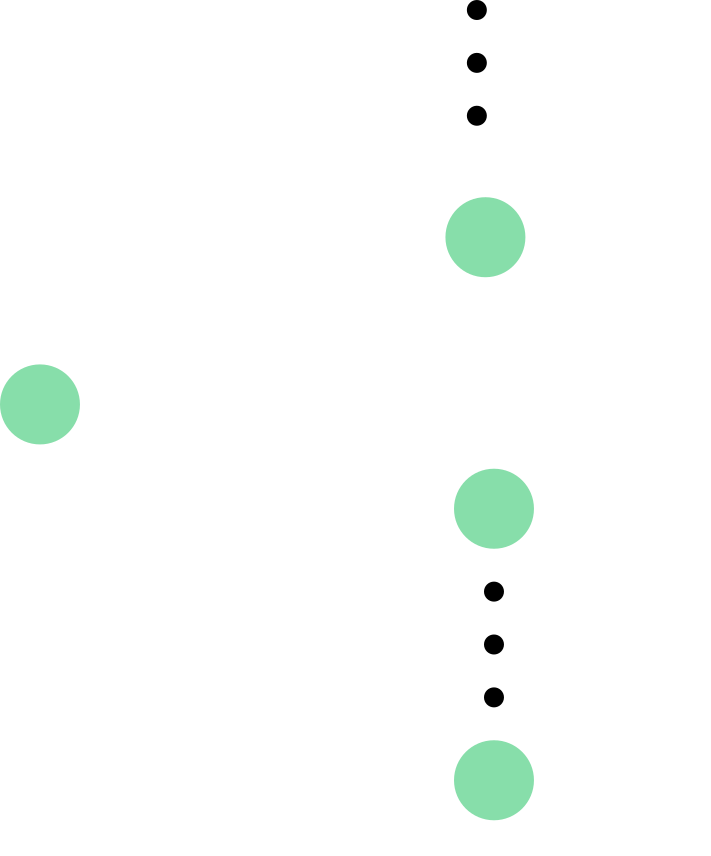
\includegraphics[width=\columnwidth]{fig/modeling-conceptual-model}
	\caption{The conceptual model.}
\end{figure}

% %
% SPECIFICATION MODEL
% %
\paragraph{Specification Model}
The state of the system is represented by the pair $(n_{cld},n_{clt})$, where $n_{cld}$ is the number of tasks in Cloudlet and $n_{cld}$ is the number of tasks in Cloud.
Tasks belonging to the first class, i.e. $t\in C_{1}$ arrive to the system with an exponential arrival process with rate $ \lambda_{1}$; whilst tasks belonging to the seconds class, i.e. $t\in C_{2}$ arrive to the system with an exponential arrival process with rate $ \lambda_{2}$.
The Cloudlet serves tasks belonging to the first class with exponentially distributed service time with rate $\mu_{cld,1}$; whilst the Cloudlet serves tasks belonging to the second class with exponentially distributed service time with rate $\mu_{cld,2}$.
The Cloud serves tasks belonging to the first class with exponentially distributed service time with rate $\mu_{clt,1}$; whilst the Cloudlet serves tasks belonging to the second class with exponentially distributed service time with rate $\mu_{clt,2}$.
We assume that 
(i) $\mu_{clt,i}>\mu_{cld,i}\ \forall i=1,2$ and
(ii) the setup time $T_{setup}$ is exponentially distributed with expected value $E[T_{setup}]$.

% %
% COMPUTATIONAL MODEL
% %
\paragraph{Computational Model}
The proposed performance model has been implemented as a Python application. 
The simulation parameters can be configured with a simple YAML file that can be loaded by the simulation program.
The full open source code is available at \cite{gmarciani-demule} and some representative configurations and outputs are presented in Section \ref{sec:usage}.

As the model follows the next-event simulation paradigm, a custom multi-stream Lehmer generator has been used to generate random events, whose parameters have been described in Section \ref{sec:random-number-generation} and whose evaluation will be presented in Section \ref{sec:evaluation}.


% %
% VERIFICATION
% %
\paragraph{Verification}
The model has been verified by checking the flow balance condition and the consistent variation of output statistics, e.g. system utilization, when varying workload rates.

% %
% VALIDATION
% %
\paragraph{Validation}
It is well-known that model development should includes a final validation step. Clearly, we cannot conduct this final step because we cannot compare the performance model with its real counterpart.